\chapter{Betriebsschwingungsanalyse}
\label{sec: Hauptkapitel 2}


\section{Aufgabenstellung}
%=========================
    % Grundziel
    %----------
    Ziel dieser Laboraufgabe ist das Durchführen einer Betriebsschwingungsanalyse
    mit anschließender Erstellung eines Campbell-Diagramms. Der Motor des
    Modellflugzeugs soll dabei von einem Elektromotor ohne Verdichtung
    geschleppt werden. Das Schwingungssignal soll an einem bestimmten Punkt der
    Tragfläche abgenommen werden.
%================================================================================

\section{Versuchsaufbau}
%=======================
    % Sensorplatzierung
    %------------------
    Obwohl nur ein Sensorsignal ausgewertet werden muss, werden 4
    Beschleunigungssensoren am vorderen Tragflügel positioniert platziert.
    Somit kann mit einem Aufbau und einer Messung sowohl die Aufgabe von Kapitel
    \ref{sec: Hauptkapitel 2} und Kaptiel \ref{sec: Hauptkapitel 3}
    abgewickelt werden. Die Beschleunigungssensoren werden an Punkten 1, 2, 4 und
    5 rot platziert (siehe Abbildung \ref{fig: Sensorpos_BSA}). Im Zuge von
    Kapitel \ref{sec: Hauptkapitel 2} wird der Messpunkt 5 rot verwendet und in
    weiterer Folge als Messpunkt 1 bezeichnet.

    % Bild - Sensorplatzierung BSA
    %-----------------------------
    \begin{figure}[H]
        \centering
        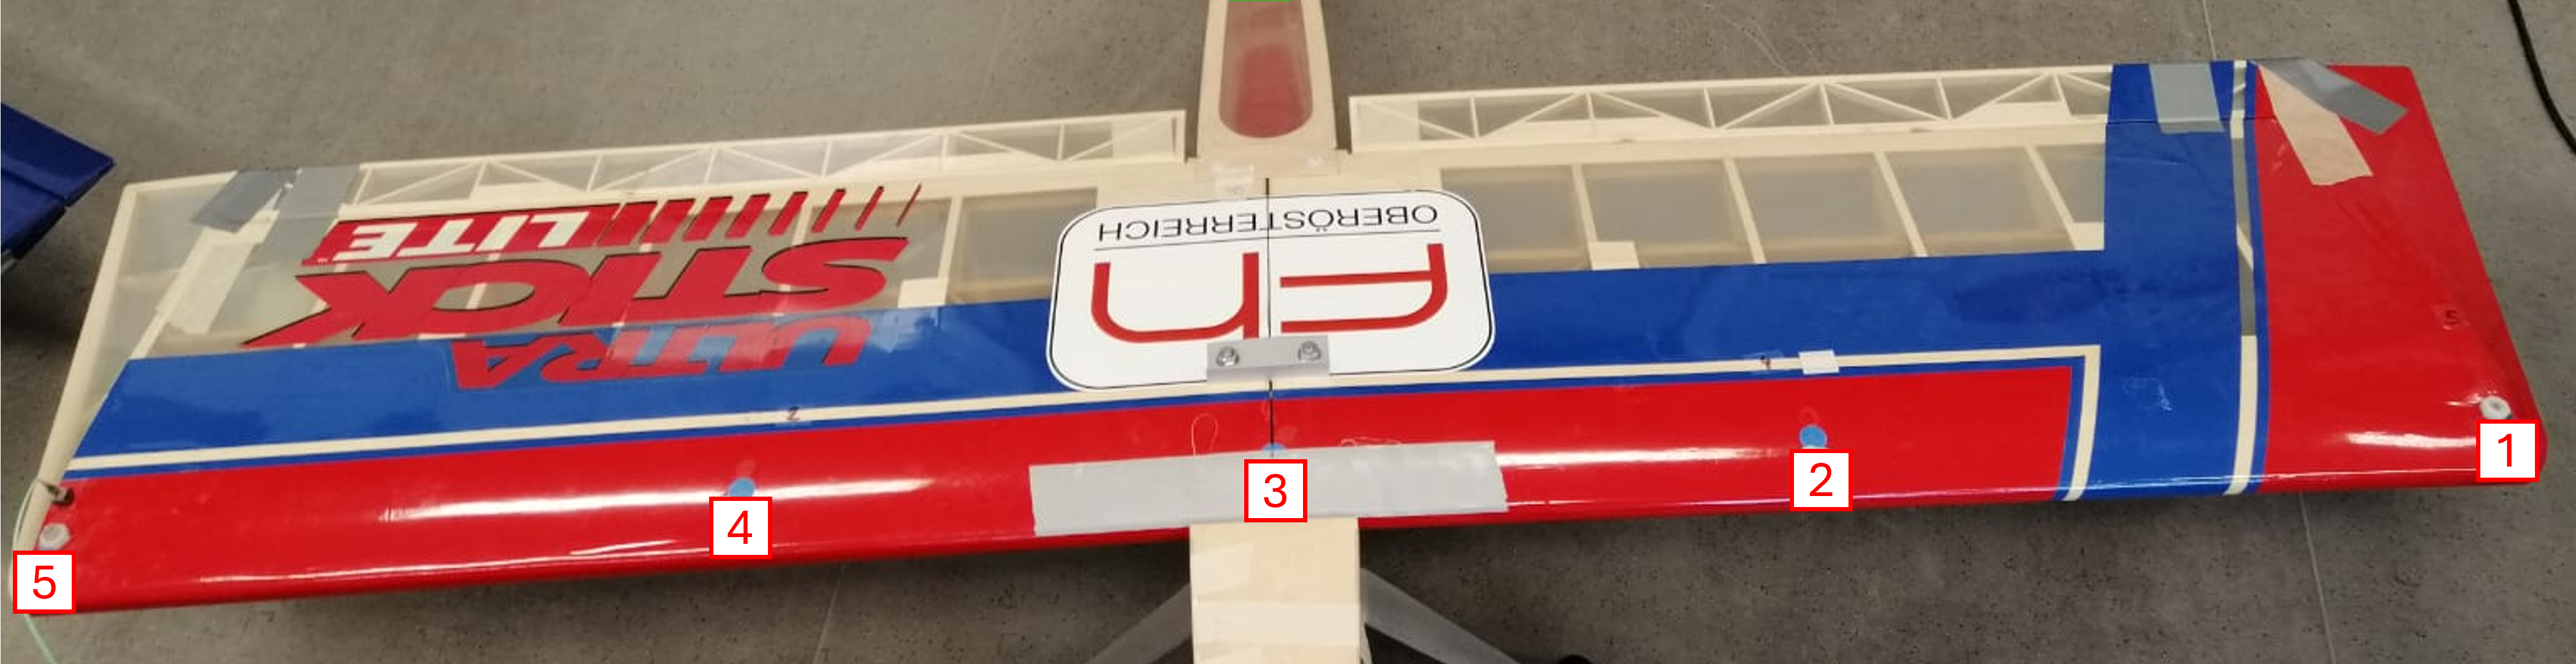
\includegraphics[width=0.9\textwidth]{BSA_Sensorpositionen.png}
        \caption{Sensorpositionen BSA}
        \label{fig: Sensorpos_BSA}
    \end{figure}
    %----------------------------------------------------------------------------

    % Fixierung Flieger
    %------------------
    \noindent
    Damit der Modellflieger bei den Messungen nicht durch die Schwingungen
    verfahren wird, wird er am Boden fixiert. Dazu werden behelfsmäßige Keile mit
    Klebeband am Boden bei den Rädern befestigt.
    \\
    %----------------------------------------------------------------------------

    % Messung mit Motor
    %------------------
    \noindent
    Bevor nun die Betriebsschwingungsanalyse durchgeführt werden kann, wird der
    Motor des Modellflugzeugs mit etwas Öl geschmiert. Dann wird der Elektromotor
    an die Welle zum Übertragen des Drehmoments angesetzt. Nun kann die Messung
    gestartet werden. Dabei wird der Elektromotor langsam mit einer Rampe von einer
    Spannung von 0 [V] auf 5 [V] beschleunigt. 

%================================================================================

\section{Ergebnisse}


